\chapter{Implementacja}

\def \noderadius {1.2cm}
\def \noderadiuspt {0.6}
\def \radius {1.5}
\def \marginangle {30}

% on-the-fly
% w wezlach wartosc MAP oryginalna i po algorytmie

% uda sie, wracamy do akceptujacego
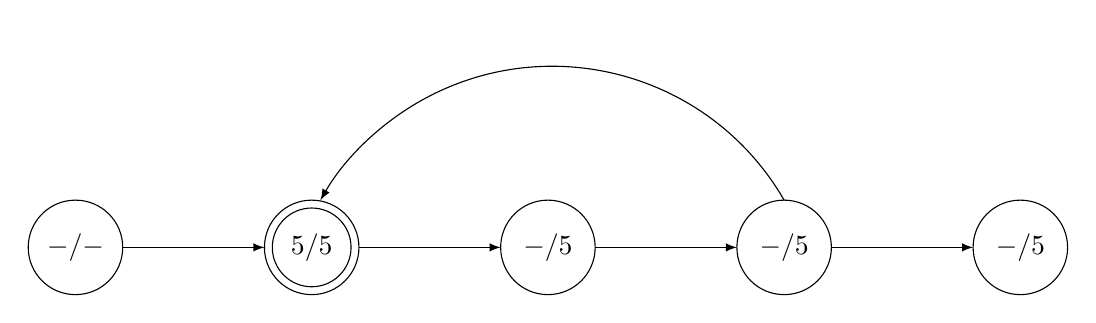
\begin{tikzpicture}
\draw (-4,0) node[draw, circle, minimum size=\noderadius] {$-/-$};
\draw[->, >=latex] (-4+\noderadiuspt,0) -- (-1-\noderadiuspt,0);
\draw (-1,0) node[draw, circle, minimum size=\noderadius] {$5/5$};
\draw (-1,0) node[draw, circle, minimum size=\noderadius-0.2cm] {};
\draw[->, >=latex] (-1+\noderadiuspt,0) -- (2-\noderadiuspt,0);
\draw (2,0) node[draw, circle, minimum size=\noderadius] {$-/5$};
\draw[->, >=latex] (2+\noderadiuspt,0) -- (5-\noderadiuspt,0);
\draw (5,0) node[draw, circle, minimum size=\noderadius] {$-/5$};
\draw[->, >=latex] (5+\noderadiuspt,0) -- (8-\noderadiuspt,0);
\draw (8,0) node[draw, circle, minimum size=\noderadius] {$-/5$};
\draw[->, >=latex] (5,\noderadius/2) arc ({\marginangle}:{180 - \marginangle}:3.4);
\end{tikzpicture}

% uda sie, wartosc MAP ze stanu 2 przeszla na 3 i 4
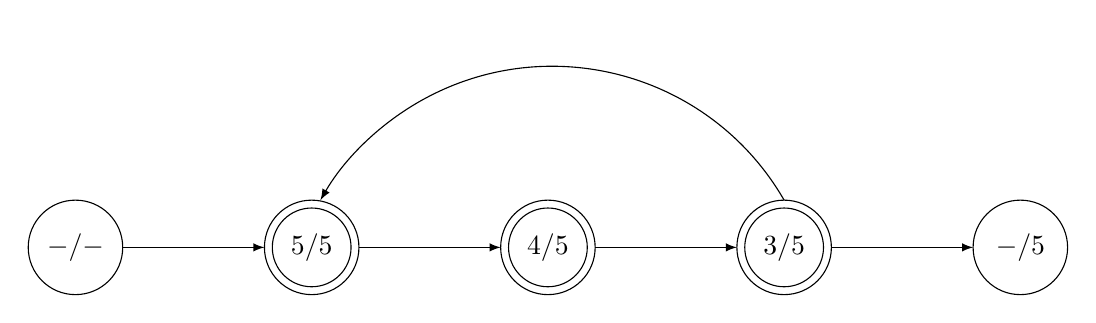
\begin{tikzpicture}
\draw (-4,0) node[draw, circle, minimum size=\noderadius] {$-/-$}; % null,null
\draw[->, >=latex] (-4+\noderadiuspt,0) -- (-1-\noderadiuspt,0);
\draw (-1,0) node[draw, circle, minimum size=\noderadius] {$5/5$}; % 5,5
\draw (-1,0) node[draw, circle, minimum size=\noderadius-0.2cm] {};
\draw[->, >=latex] (-1+\noderadiuspt,0) -- (2-\noderadiuspt,0);
\draw (2,0) node[draw, circle, minimum size=\noderadius] {$4/5$}; % 4,5
\draw (2,0) node[draw, circle, minimum size=\noderadius-0.2cm] {};
\draw[->, >=latex] (2+\noderadiuspt,0) -- (5-\noderadiuspt,0);
\draw (5,0) node[draw, circle, minimum size=\noderadius] {$3/5$}; % 3,5
\draw (5,0) node[draw, circle, minimum size=\noderadius-0.2cm] {};
\draw[->, >=latex] (5+\noderadiuspt,0) -- (8-\noderadiuspt,0);
\draw (8,0) node[draw, circle, minimum size=\noderadius] {$-/5$}; % null,5
\draw[->, >=latex] (5,\noderadius/2) arc ({\marginangle}:{180 - \marginangle}:3.4);
\end{tikzpicture}

% nie uda się -> kolejne stany akceptujące mają wiekszą wartość MAP, przez co poprzednia zostaje zapomniana
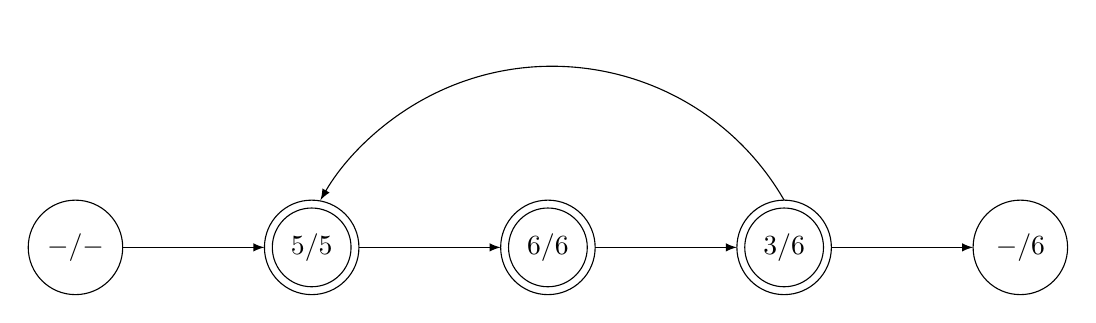
\begin{tikzpicture}
\draw (-4,0) node[draw, circle, minimum size=\noderadius] {$-/-$}; % null,null
\draw[->, >=latex] (-4+\noderadiuspt,0) -- (-1-\noderadiuspt,0);
\draw (-1,0) node[draw, circle, minimum size=\noderadius] {$5/5$}; % 5,5
\draw (-1,0) node[draw, circle, minimum size=\noderadius-0.2cm] {};
\draw[->, >=latex] (-1+\noderadiuspt,0) -- (2-\noderadiuspt,0);
\draw (2,0) node[draw, circle, minimum size=\noderadius] {$6/6$}; % 6,6
\draw (2,0) node[draw, circle, minimum size=\noderadius-0.2cm] {};
\draw[->, >=latex] (2+\noderadiuspt,0) -- (5-\noderadiuspt,0);
\draw (5,0) node[draw, circle, minimum size=\noderadius] {$3/6$}; % 3,6
\draw (5,0) node[draw, circle, minimum size=\noderadius-0.2cm] {};
\draw[->, >=latex] (5+\noderadiuspt,0) -- (8-\noderadiuspt,0);
\draw (8,0) node[draw, circle, minimum size=\noderadius] {$-/6$}; % null,6
\draw[->, >=latex] (5,\noderadius/2) arc ({\marginangle}:{180 - \marginangle}:3.4);
\end{tikzpicture}

% nie uda sie -> mimo poprawnej pętli, stan 3 nie jest źródłem wartości propagowanej dalej
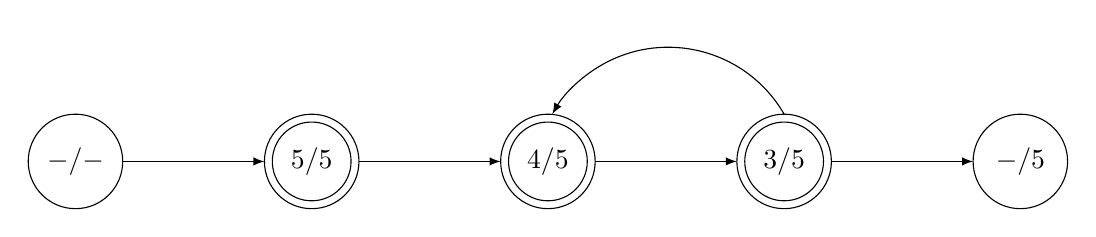
\begin{tikzpicture}
\draw (-4,0) node[draw, circle, minimum size=\noderadius] {$-/-$};
\draw[->, >=latex] (-4+\noderadiuspt,0) -- (-1-\noderadiuspt,0);
\draw (-1,0) node[draw, circle, minimum size=\noderadius] {$5/5$};
\draw (-1,0) node[draw, circle, minimum size=\noderadius-0.2cm] {};
\draw[->, >=latex] (-1+\noderadiuspt,0) -- (2-\noderadiuspt,0);
\draw (2,0) node[draw, circle, minimum size=\noderadius] {$4/5$};
\draw (2,0) node[draw, circle, minimum size=\noderadius-0.2cm] {};
\draw[->, >=latex] (2+\noderadiuspt,0) -- (5-\noderadiuspt,0);
\draw (5,0) node[draw, circle, minimum size=\noderadius] {$3/5$};
\draw (5,0) node[draw, circle, minimum size=\noderadius-0.2cm] {};
\draw[->, >=latex] (5+\noderadiuspt,0) -- (8-\noderadiuspt,0);
\draw (8,0) node[draw, circle, minimum size=\noderadius] {$-/5$};
\draw[->, >=latex] (5,\noderadius/2) arc ({\marginangle}:{180 - \marginangle}:1.7);
\end{tikzpicture}


% TODO opisac funkcje globalne: getInitialStates(), isAccepting(x), acceptingCycleFound()
\begin{algorithm}
\caption{$ detectAcceptingCycle() $}
\begin{algorithmic}[1]
\REQUIRE $ G = (V,E,ACC) $

\STATE $ initialStates \leftarrow getInitialStates() $
\STATE $ approximationSet \leftarrow initialise(initialStates) $
\STATE $ oldSize \leftarrow \infty $
\WHILE{$ (approximationSet.size \neq oldSize)\ \mathbf{and}\ (approximationSet.size > 0) $}
  \STATE $ oldSize \leftarrow approximationSet.size $
  \STATE $ eliminateNoAccepting(approximationSet) $
  \STATE $ eliminateNoPredecessors(approximationSet) $
\ENDWHILE
\RETURN $ approximationSet.size > 0 $
\end{algorithmic}
\end{algorithm}


\begin{algorithm}
\caption{$ initialise(initialStates) $}
\begin{algorithmic}[1]
\REQUIRE $ initialStates $

\STATE $ approximationSet \leftarrow initialStates $
\STATE $ q \leftarrow new\ Queue() $
\STATE $ q.pushBack(initialStates) $
\WHILE{$ q.isNotEmpty() $}
  \STATE $ s \leftarrow q.popFront() $
  \FORALL{$ t \in getSuccessors(s) $}
    \IF{$ t \notin approximationSet $}
      \STATE $ approximationSet.add(t) $
      \STATE $ q.pushBack(t) $
    \ENDIF
    \IF{$ isAccepting(t) $}
      \IF{$ (t == s)\ \mathbf{or}\ (approximationSet.getMap(s) == t) $}
        \STATE $ acceptingCycleFound() $
        \RETURN
      \ENDIF
      \STATE $ approximationSet.setMap(t, max(t, approximationSet.getMap(s))) $
    \ELSE
      \STATE $ approximationSet.setMap(t, approximationSet.getMap(s)) $
    \ENDIF
  \ENDFOR
\ENDWHILE
\RETURN $ approximationSet $
\end{algorithmic}
\end{algorithm}


\begin{algorithm}
\caption{$ eliminateNoAccepting(approximationSet) $}
\begin{algorithmic}[1]
\REQUIRE $ approximationSet $

\STATE $ tmpApproximationSet \leftarrow \emptyset $
\STATE $ q \leftarrow new\ Queue() $
\FORALL{$ s \in approximationSet $}
  \IF{$ isAccepting(s) $}
    \STATE $ q.pushBack(s) $
    \STATE $ tmpApproximationSet.add(s) $
    \STATE $ tmpApproximationSet.setPredecessorCount(s,0) $
  \ENDIF
\ENDFOR
\STATE $ approximationSet \leftarrow tmpApproximationSet $
\WHILE{$ q.isNotEmpty() $}
  \STATE $ s \leftarrow q.popFront() $
  \FORALL{$ t \in getSuccessors(s) $}
    \IF{$ t \in approximationSet $}
      \STATE $ approximationSet.incrementPredecessorCount(t) $
    \ELSE
      \STATE $ q.pushBack(t) $
      \STATE $ approximationSet.add(t) $
      \STATE $ approximationSet.setPredecessorCount(t,0) $
    \ENDIF
  \ENDFOR
\ENDWHILE
\end{algorithmic}
\end{algorithm}


\begin{algorithm}
\caption{$ eliminateNoPredecessors(approximationSet) $}
\begin{algorithmic}[1]
\REQUIRE $ approximationSet $

\STATE $ q \leftarrow new\ Queue() $
\FORALL{$ s \in approximationSet $}
  \IF{$ approximationSet.getPredecessorCount(s) == 0 $}
    \STATE $ q.pushBack(s) $
  \ENDIF
\ENDFOR
\WHILE{$ q.isNotEmpty() $}
  \STATE $ s \leftarrow q.popFront() $
  \STATE $ approximationSet.remove(s) $
  \FORALL{$ t \in getSuccessors(s) $}
    \STATE $ approximationSet.decrementPredecessorCount(t) $
    \IF{$ approximationSet.getPredecessorCount(t) == 0 $}
      \STATE $ q.pushBack(t) $
    \ENDIF
  \ENDFOR
\ENDWHILE
\end{algorithmic}
\end{algorithm}



\section{Ignore}

TODO

przestrzen stanow, automaty, automaty buchiego (przykladowe obrazki automatow z podanej formuly LTL, opis ze potrzebna negacja i szukanie spelnialnosci)
weryfikacja hardware i software
alogrytmy wykorzystywane w przeszukiwaniu i weryfikacji
co to i po co on-the-fly
Alvis, co to, po co

przejrzec publikacje profesora


w czesci implementacji:
opis weryfikowanego systemu


A time-optimal on-the-fly parallel algorithm for model checking of weak LTL properties, in: Formal Methods and Software Engineering
